\newpage
\section{Auswertung}
\label{sec:Auswertung}

\subsection{Messung des Schwellstroms}
\label{sec:schwellstrom}

Der Schwellstrom wird wie in Kapittel \ref{sec:schwellenstrom} beschrieben ermittelt. 
Von der Detektorkarte wird je ein Bild kurz vor erreichen des Schwellstroms, als auch kurz danach gemacht.
Diese Bilder sind in Abbildung  \ref{fig:1} zu finden.
Der Schwellstrom wird auf $I_{\text{thr}} = \SI{48}{\milli\ampere}$ bestimmt.

\begin{figure}
    \centering
    \begin{subfigure}[b]{0.49\textwidth}
        \centering
        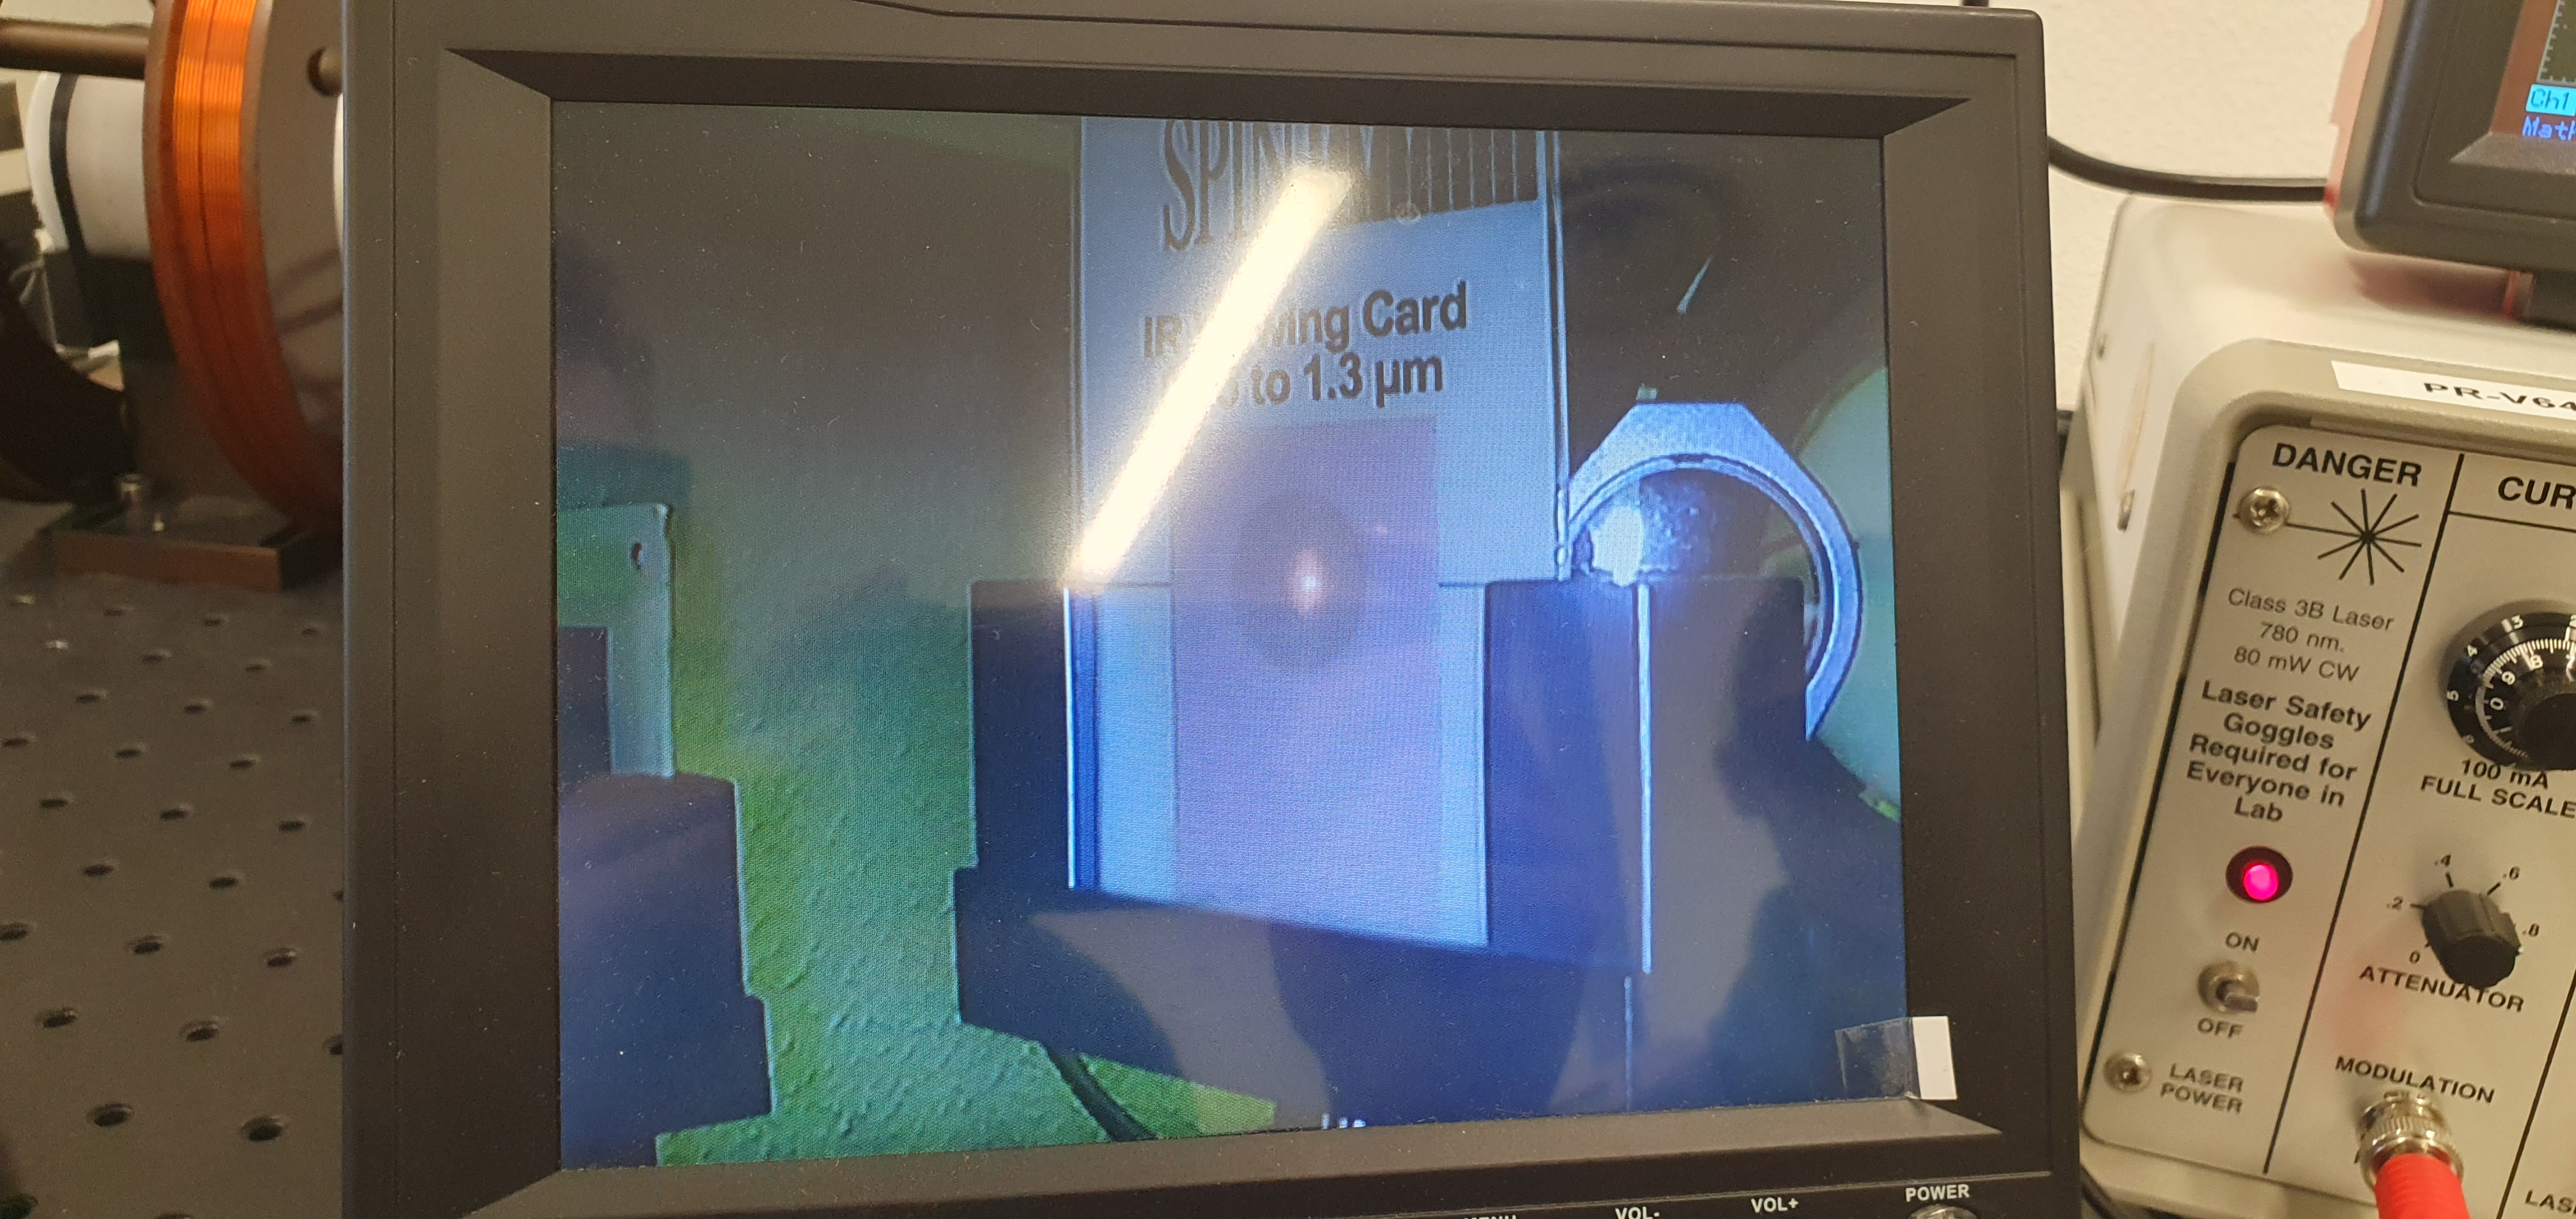
\includegraphics[width= \textwidth]{plots/Schwellstrom_1.jpg}
    \end{subfigure}
    \hfill
    \begin{subfigure}[b]{0.49\textwidth}
        \centering
        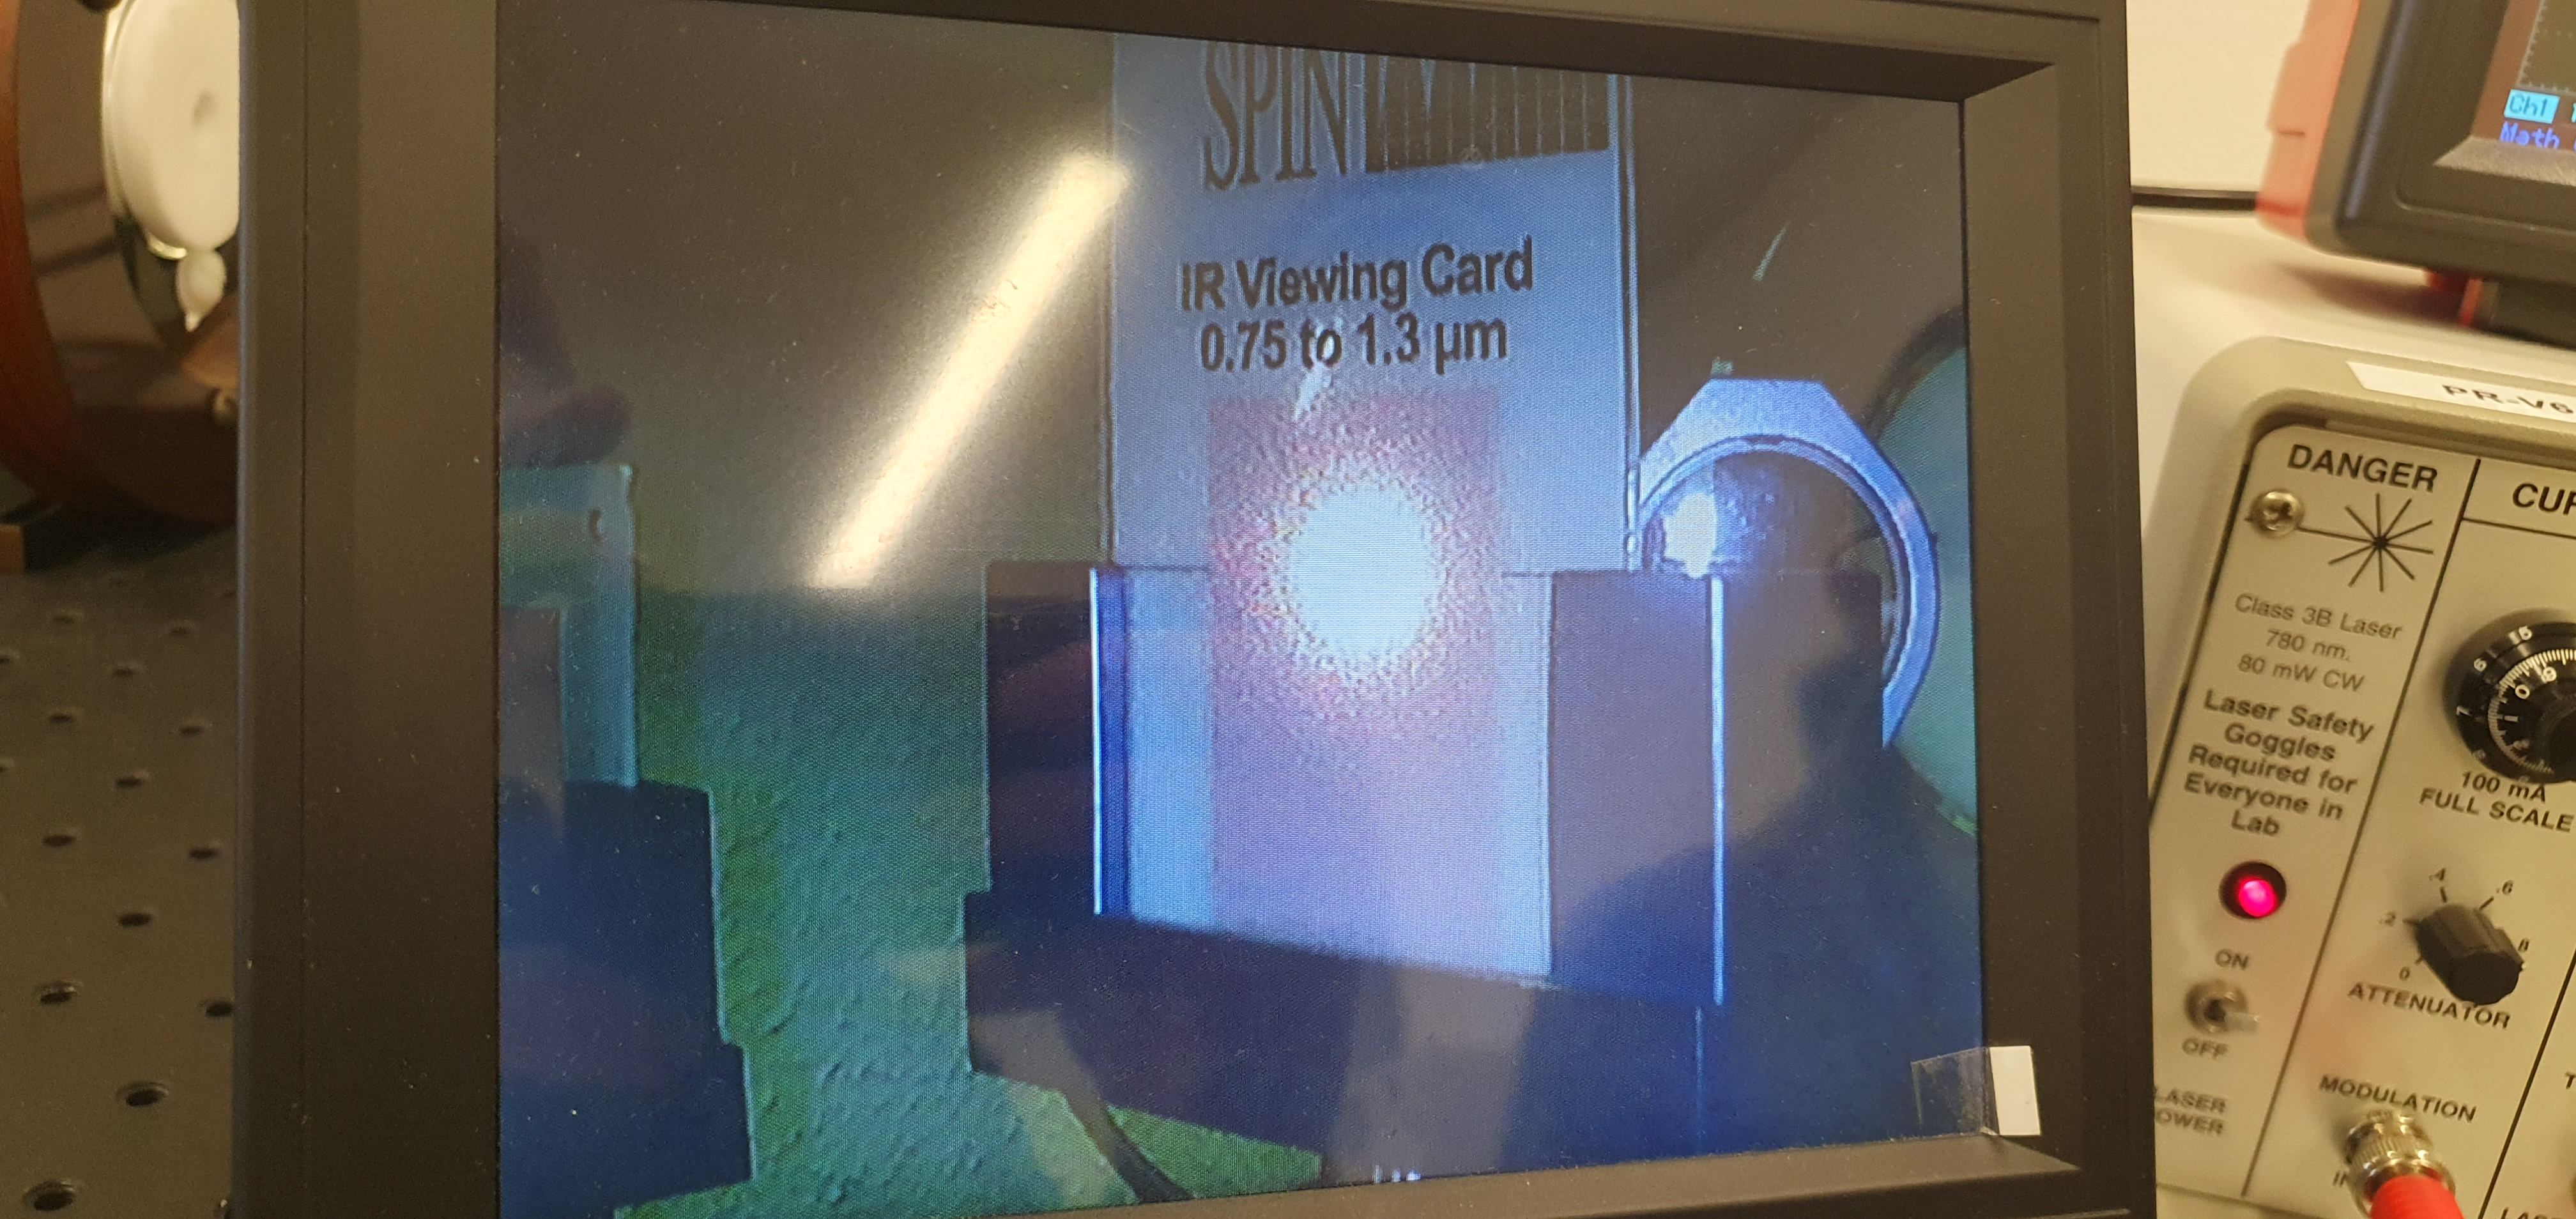
\includegraphics[width= \textwidth]{plots/Schwellstrom_2.jpg}
    \end{subfigure}
    \caption{Bild der Detektorkarte, kurz bevor (links) und kurz nachdem (rechts) der Schwellstrom erreicht worden ist.}
    \label{fig:1}
\end{figure}


\subsection{Rubidiumfluoreszenz und Transmissionsspektrum}

Um die Rubidiumfluoreszenz zu sehen, wird wie in Kapittel \ref{sec:Rubidium} beschrieben vorgegangen.
Der verwendete Strom beträgt \SI{62.4}{\milli\ampere} und der Piezo-Kristall ist eingeschaltet.
Die Rubidiumfluoreszenz ist in Abbildung \ref{fig:2} zu sehen.
Das Transmissionsspektrum ist in Abbildung \ref{fig:3} zu sehen.
Dabei sind deutlich vier Absorptionslinien des Rubidiums zu sehen. 
Durch feines Justieren wird sichergestellt, dass keine Modensprünge auftreten. 
So können die Peaks von links nach rechts den Übergängen 87a, 85a, 85b, 87b zugeordnet werden.

\begin{figure}
    \centering
    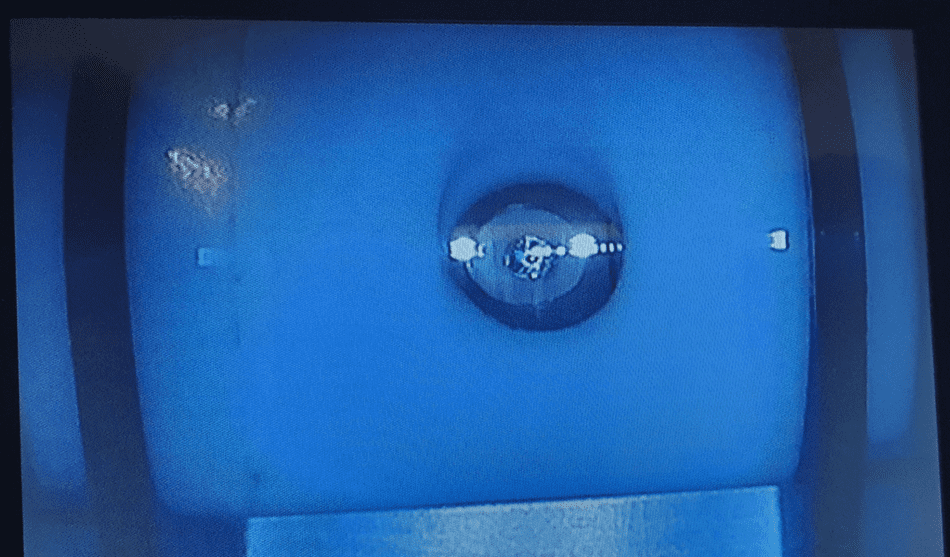
\includegraphics[width= 0.7\textwidth]{plots/Fluoreszenz_1.png}
    \caption{Bild der Radiumfluoriszenz.}
    \label{fig:2}
\end{figure}

\begin{figure}
    \centering
    \begin{subfigure}[b]{0.49\textwidth}
        \centering
        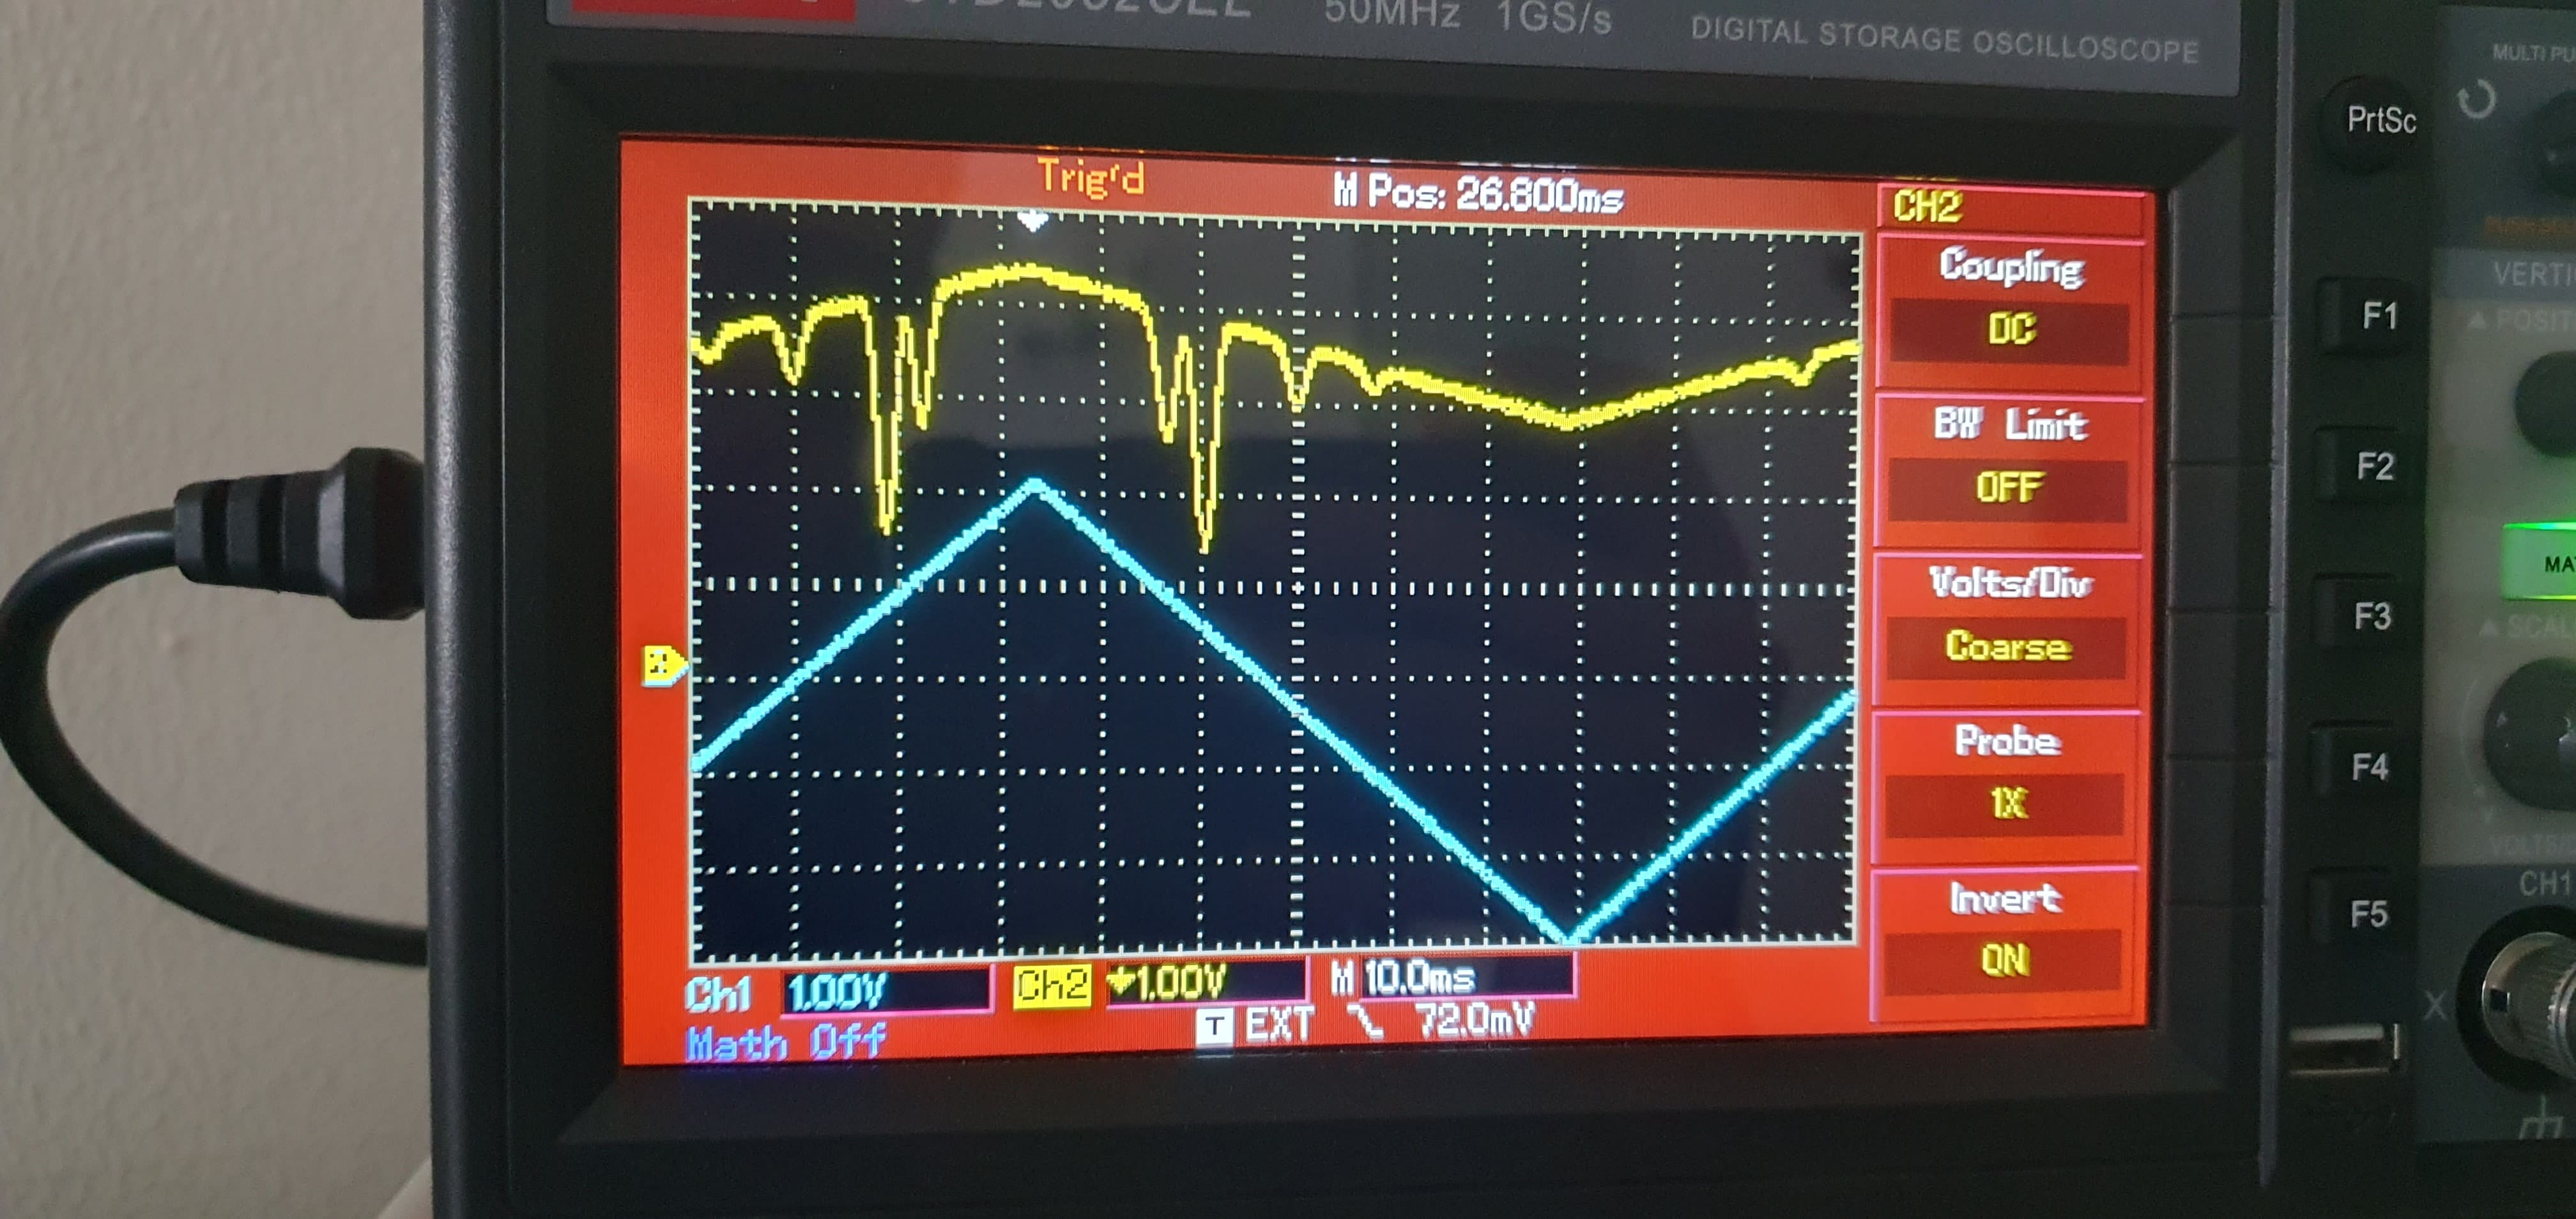
\includegraphics[width= \textwidth]{plots/Absorption_1.jpg}
    \end{subfigure}
    \hfill
    \begin{subfigure}[b]{0.49\textwidth}
        \centering
        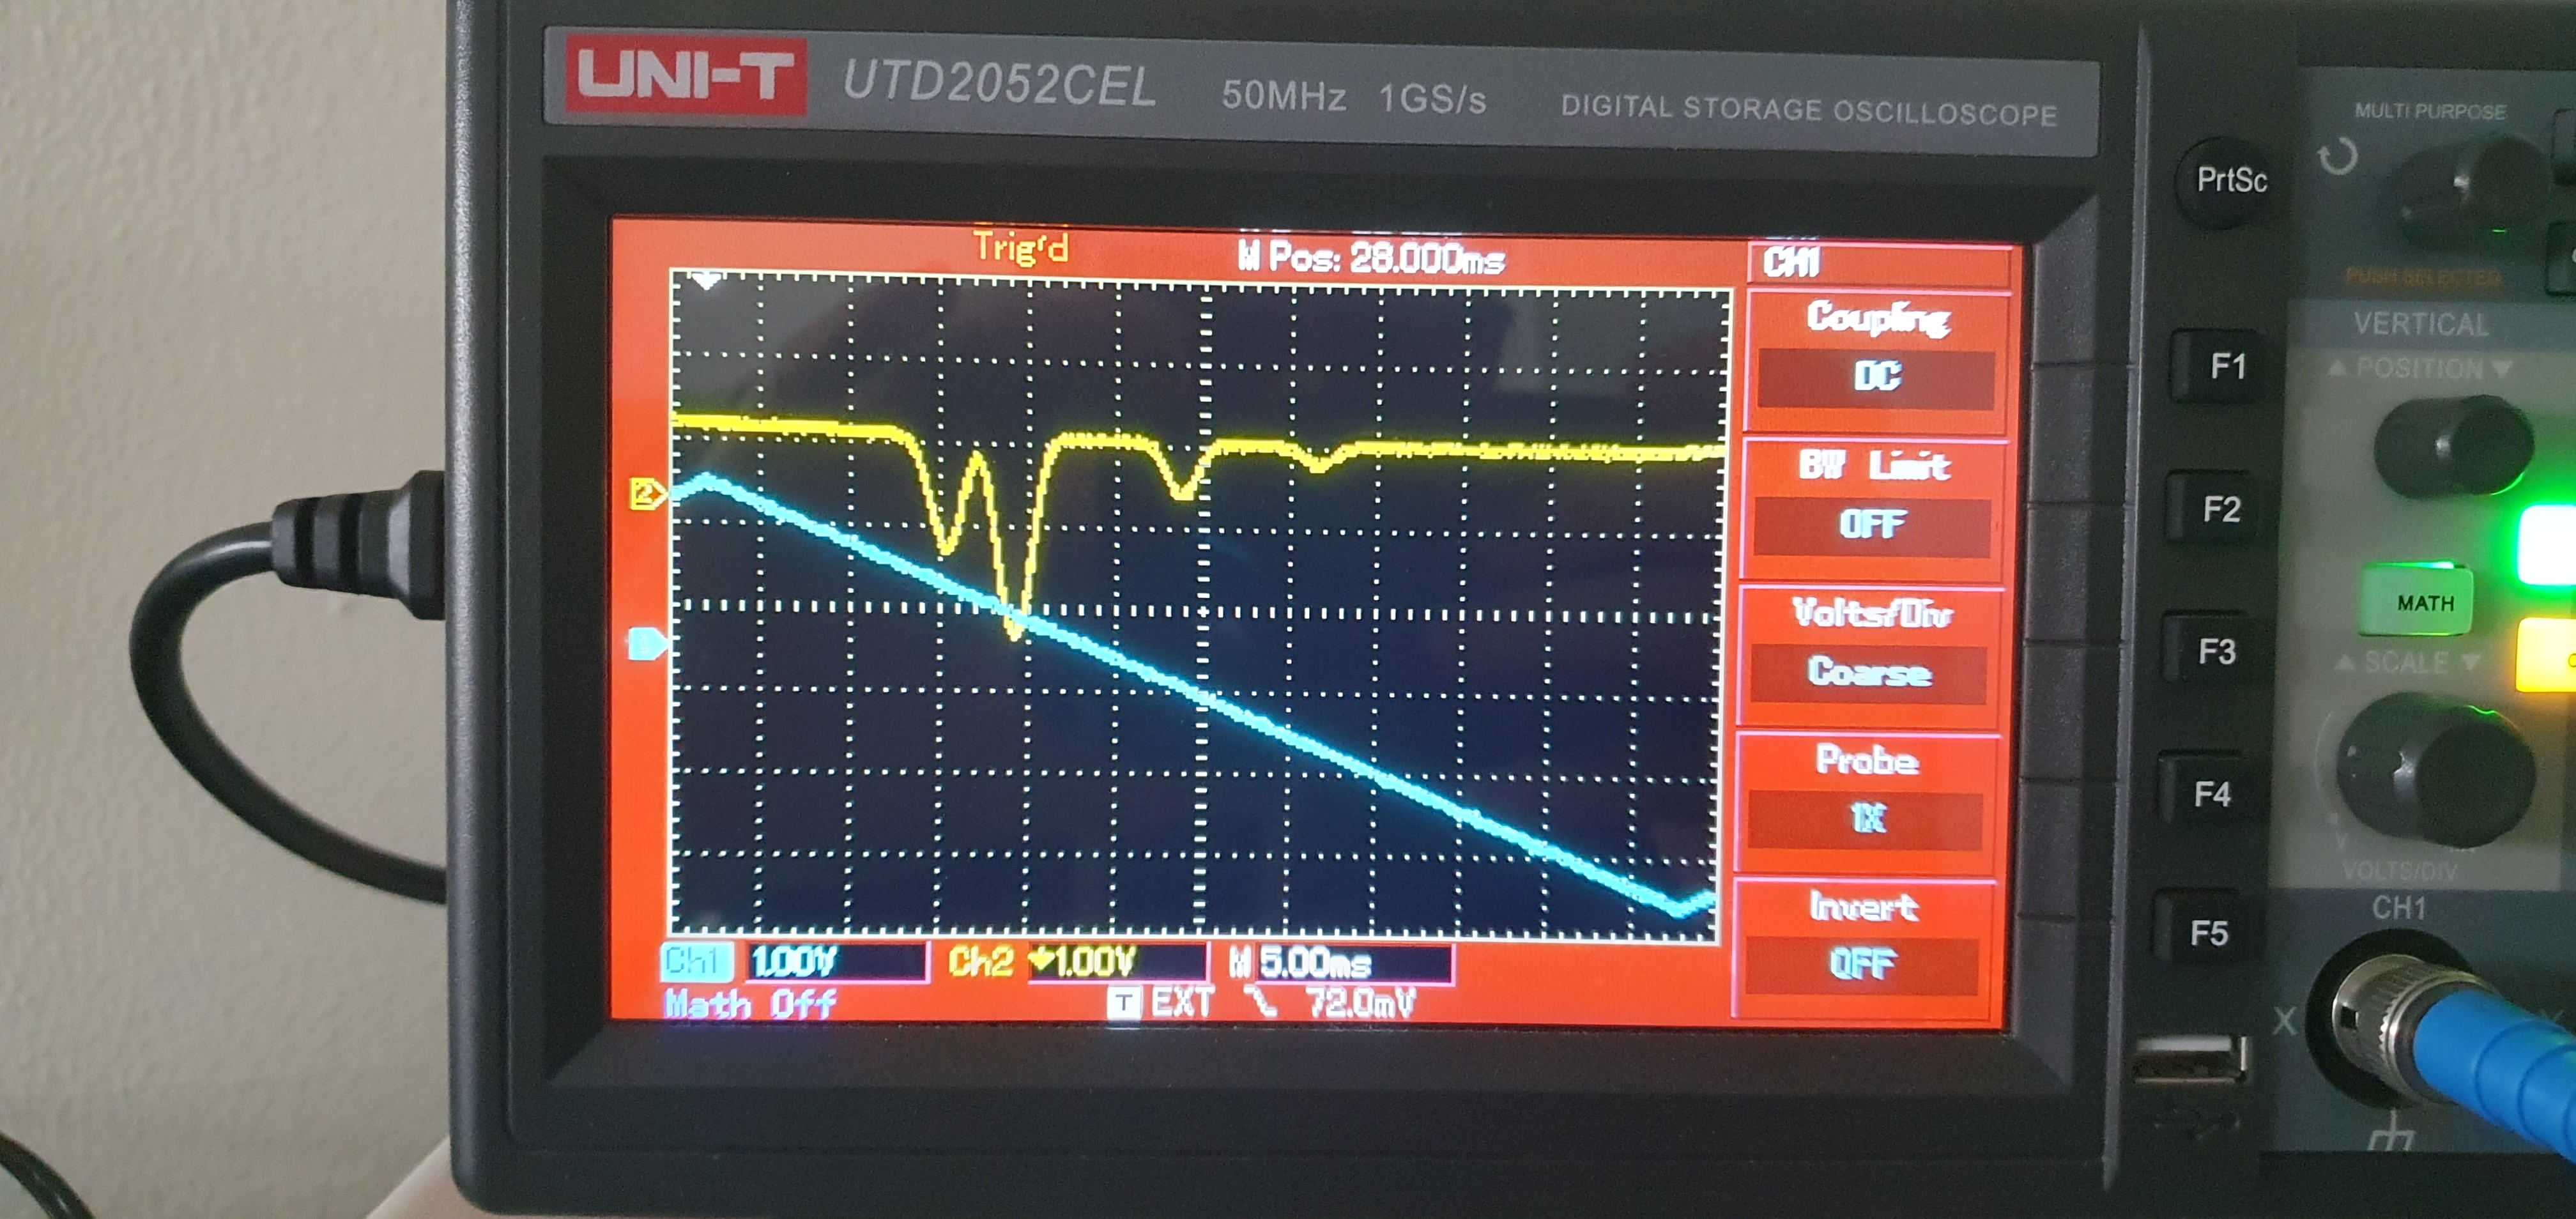
\includegraphics[width= \textwidth]{plots/Absorption_2.jpg}
    \end{subfigure}
    \caption{Das transmissionsspektrum ohne Unterdrückung des Untergrundes (links) und mit Unterdrückung des Untergrundes (rechts).}
    \label{fig:3}
\end{figure}